\subsection{Hardware implementation}\label{sec:roib_current}

The RoIB is implemented as a custom 9U VMEbus system that includes a controller which configures and monitors the system along with custom cards 
that receive and assemble the event fragments and send them to the HLT. Figure \ref{roib_run1} shows a block of the RoIB and 
its connection to external systems.
%\footnote{Note the L2 Supervisor farm from Run-1 has evolved to a commodity server PC running the HLTSV application.}.

\begin{figure}[tbp] % figures (and tables) should go top or bottom of
                    % the page where they are first cited or in
                    % subsequent pages
\centering
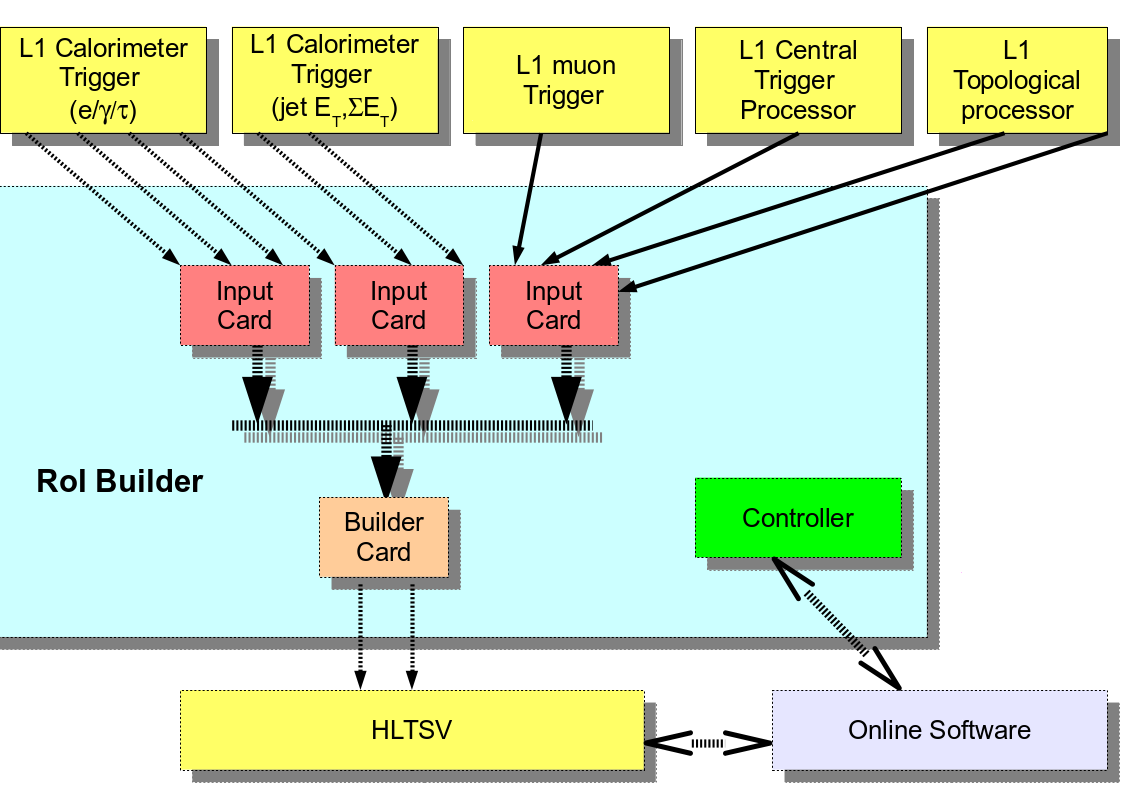
\includegraphics[width=.65\textwidth]{RoIB_context_v2.png}
\caption{Block scheme of the RoI Builder and overview of connections to external systems.  The
custom input and builder cards and the controller, a commercially available single board computer,
are installed in a single 9U VMEbus crate. The controller connects to the Control Network to interact with the rest of the 
data acquisition system.}
\label{roib_run1}
\end{figure}

The RoIB contains four input cards and uses one builder card in the Run-2 configuration. Each input card accepts three inputs from 
L1 subsystems. 
The builder card assembles the input data of the events and passes the results via two optical links 
to another receiver card in a PC running the HLT supervisor (HLTSV) application. The receiver card in the HLTSV is a TILAR card \cite{tilar}
 that implements four PCIe Gen1 lanes to interface with the two optical links. The HLTSV manages the HLT processing farm by using L1 results provided by the RoIB, retrieves events from the ROS, assigns events to HLT farm nodes, and handles event bookkeeping including requesting removal of data from ROS storage when no longer required. 

The fragments received by the RoIB are identified by a 32 bit identifier, the extended L1 ID (L1ID). 
The RoIB input cards use the L1ID and the number of outputs enabled to assign keys to the various fragments and send them to the output channel in the builder card that was 
assigned that key value. The input data is transferred over a custom J3 back-plane. The back-plane operates at 20 MHz and transfers 16 data bits per 
clock cycle simultaneously for up to 12 inputs. The total maximum data throughput is therefore 480 MB/s, 40 MB/s per input.  
The maximum size of any single fragment is limited to 512 bytes imposed by resources available in the FPGA firmware. The current RoIB input 
links are listed in Table \ref{tab:roib_links}.

\begin{table}[tbp]
\caption{L1 input sources to the RoIB.}
\label{tab:roib_links}
\smallskip
\centering
\begin{tabular}{|c|c|}
\hline
Source & Links\\
\hline
Central Trigger Processor (CTP)  & 1  \\
L1 calorimeters (e/$\gamma$, $\tau$, jet, $\sum E_\mathrm{T}$) & 6  \\
Muon Trigger to CTP Interface (MUCTPI) & 1  \\
Topological processor (L1Topo) & 2  \\
Spare & 2 \\
\hline
\end{tabular}
\end{table}

\subsection{System Performance and Evolution}\label{sec:roib_limit}

The custom VMEbus based RoIB operated reliably during the first run of the LHC, however, it is desirable to have a more flexible RoIB. 
In addition, the RoIB is getting close to its design limitation, as seen 
in Figure \ref{fig:cern_robinnproib}. For fragments of 400 bytes and inputs from eight L1 systems, referred to as channels, the current RoIB rate limit is 60 kHz which is below the required 100 kHz at 
L1. While the current fragment size coming from L1 are around 160 bytes, the sizes are expected to grow due to the increase of instantaneous 
luminosity and the complexity of L1 triggers. The current VMEbus system will be replaced by a PCI-express card hosted in the HLTSV PC with the 
possibility to upgrade the commodity hardware (e.g. ability to upgrade CPUs). 
The new configuration simplifies the readout architecture of ATLAS. The targeted rate for event building is 100 kHz over 12 input channels for 
fragment sizes in the order of 400 bytes.
